\documentclass[10pt]{exam}
\usepackage[hon]{template-for-exam}
\usepackage{endnotes,graphicx}
\usepackage{tikz,graphicx,enumitem,multicol,float,my-tikz-clipart,silence,cclicenses}
\graphicspath{{./figures/}}
\WarningFilter{latex}{Label `part}
\WarningFilter{latex}{There were multiply-defined labels}

\footer{}{\thepage}{\sc \myclass}


%\def\answer#1{\footnotetext{#1}}
%\def\myquestion{\item\stepcounter{footnote}}

\def\enoteheading{}
\def\answer#1{\endnotetext{#1}}
\def\theanswers{\theendnotes}
\def\myquestion{\item\stepcounter{endnote}}

\newenvironment{myquestions}{
  \begin{multicols*}{2}\begin{enumerate}
}{
  \end{enumerate}\end{multicols*}
}
\makeatletter
\patchcmd{\enit@setresumekeys}{\def}{\gdef}{}{}
\patchcmd{\enit@setresumekeys}{\def}{\gdef}{}{}
\makeatother

\newcommand{\myheading}[1]{\uplevel{\section*{#1}}
}
\newcommand{\mysubheading}[1]{\uplevel{\subsection*{#1}}
}

%uncomment if running Pandoc
%\renewcommand{\myheading}[1]{{\section*{#1}}}
%\renewcommand{\mysubheading}[1]{\subsection*{#1}}



%%%%%%%%%%%%%%%% Dates %%%%%%%%%%%%%%%%%%%
\def\quizday{Fri, Jan 16} % also used as HW Check A Day
\def\testday{Tue, Jan 27}

\def\one{Wed, Jan 7}
\def\two{Thu-Fri, Jan 8-9}
\def\three{Thu-Fri, Jan 8-9}
\def\four{Mon, Jan 12}
\def\five{Tue, Jan 13}
\def\six{Tue, Jan 20}
%%%%%%%%%%%%%%%%%%%%%%%%%%%%%%%%%%%%%%%%%



\def\mytitle{Chapter 8 Homework (Momentum)}
\title{\mytitle}
\date{\today}

\def\mymaketitle{
  \begin{flushleft}
    {\LARGE \textbf \mytitle \par}
  \end{flushleft}
}

\newcommand{\bs}[2]{\textbf{#1} (\sc #2 Points)}


\begin{document}
\maketitle


\begin{center}
  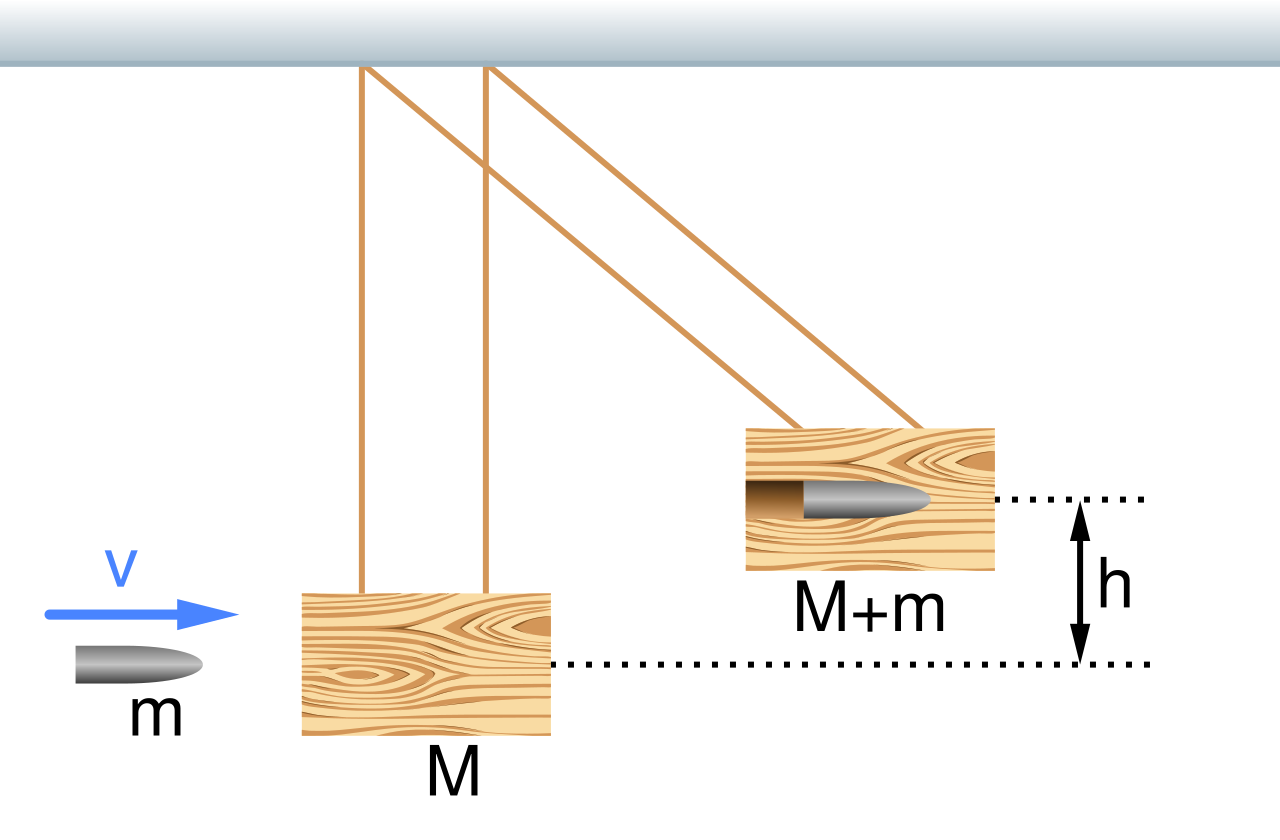
\includegraphics[height=4.1cm]{ballistic-pend.png}
  
  {\small``Sketch of a ballistic pendulum before and after it is struck by a bullet'' by \texttt{MikeRun}} 
  
  \cc\hspace{-1em}\ccby\hspace{-.7em}\ccsa  {\small CC BY-SA 4.0}
  
\end{center}

\section*{HW Check A (collected on \quizday)}


%%%%%%%%%%%

\subsection*{Reading}

Please read the following on your own in the OpenStax textbook by the dates given.  It will give good context for class discussion.  Check off when you have completed them.

\vspace{1em}

\begin{checkboxes}
  \choice 8.1 Linear Momentum \& Force \dotfill \one
  \choice 8.2 Impulse \dotfill \two
  \choice 8.3 Conservation of Momentum \dotfill \three
  \choice 8.4 Elastic Collisions in One Dimension  \dotfill \four
\end{checkboxes}


\subsection*{Problems and Conceptual Question}


Get stamps from your instructor as you complete each of the following problems.  The conceptual questions (CQ) require at least one sentence of explanation.

\vspace{1em}

\noindent
{\sc Stamps will not be given if work is not shown on a separate sheet of paper}

\vspace{1em}


\begin{tabular}{|*{3}{p{4.8cm}|}}
  \hline
  %
  \bs{Momentum}{7}               
                    & \bs{Force \& Impulse}{3}
                                      & \bs{Elastic Collisions}{5}  \\
  Problems \#\ref{1p-i}-\ref{1p-f}
              & Problems \#\ref{2p-i}-\ref{2p-f} 
                    & Problems \#\ref{4p-i}-\ref{4p-f}\\
  Conceptual \#\ref{1q-i}-\ref{1q-f}
          & Conceptual \#\ref{2q-i}-\ref{2q-f}
              & Conceptual \#\ref{4q-i}-\ref{4q-f} \\
          &   & \textbf{HW Quiz on \quizday} \\[4em]\hline
  %%

\end{tabular}

\pagebreak

\newcommand{\refsheet}{
  \section*{Equations}


  \begin{align*}
    p &\equiv mv &
    J &\equiv F\Delta t &
    \Sigma F &= \frac{\Delta p}{\Delta t} &
    \Sigma p &= \Sigma p ' &
    v_A + v_A' &= v_B + v_B' &
    x_{CM} &= \frac{\Sigma m_i x_i}{\Sigma m_i}
  \end{align*}


  \section*{Selected Answers}

  \renewcommand{\enotesize}{\normalsize}
  \renewcommand{\enoteformat}{%
    \leftskip=1.8em
    \makebox[0pt][r]{\theenmark. }%
  }

  \hfill
  \theanswers
}

\refsheet



\pagebreak
\mymaketitle
\section*{HW Check B (collected on Test Day - \testday)}

\begin{center}
  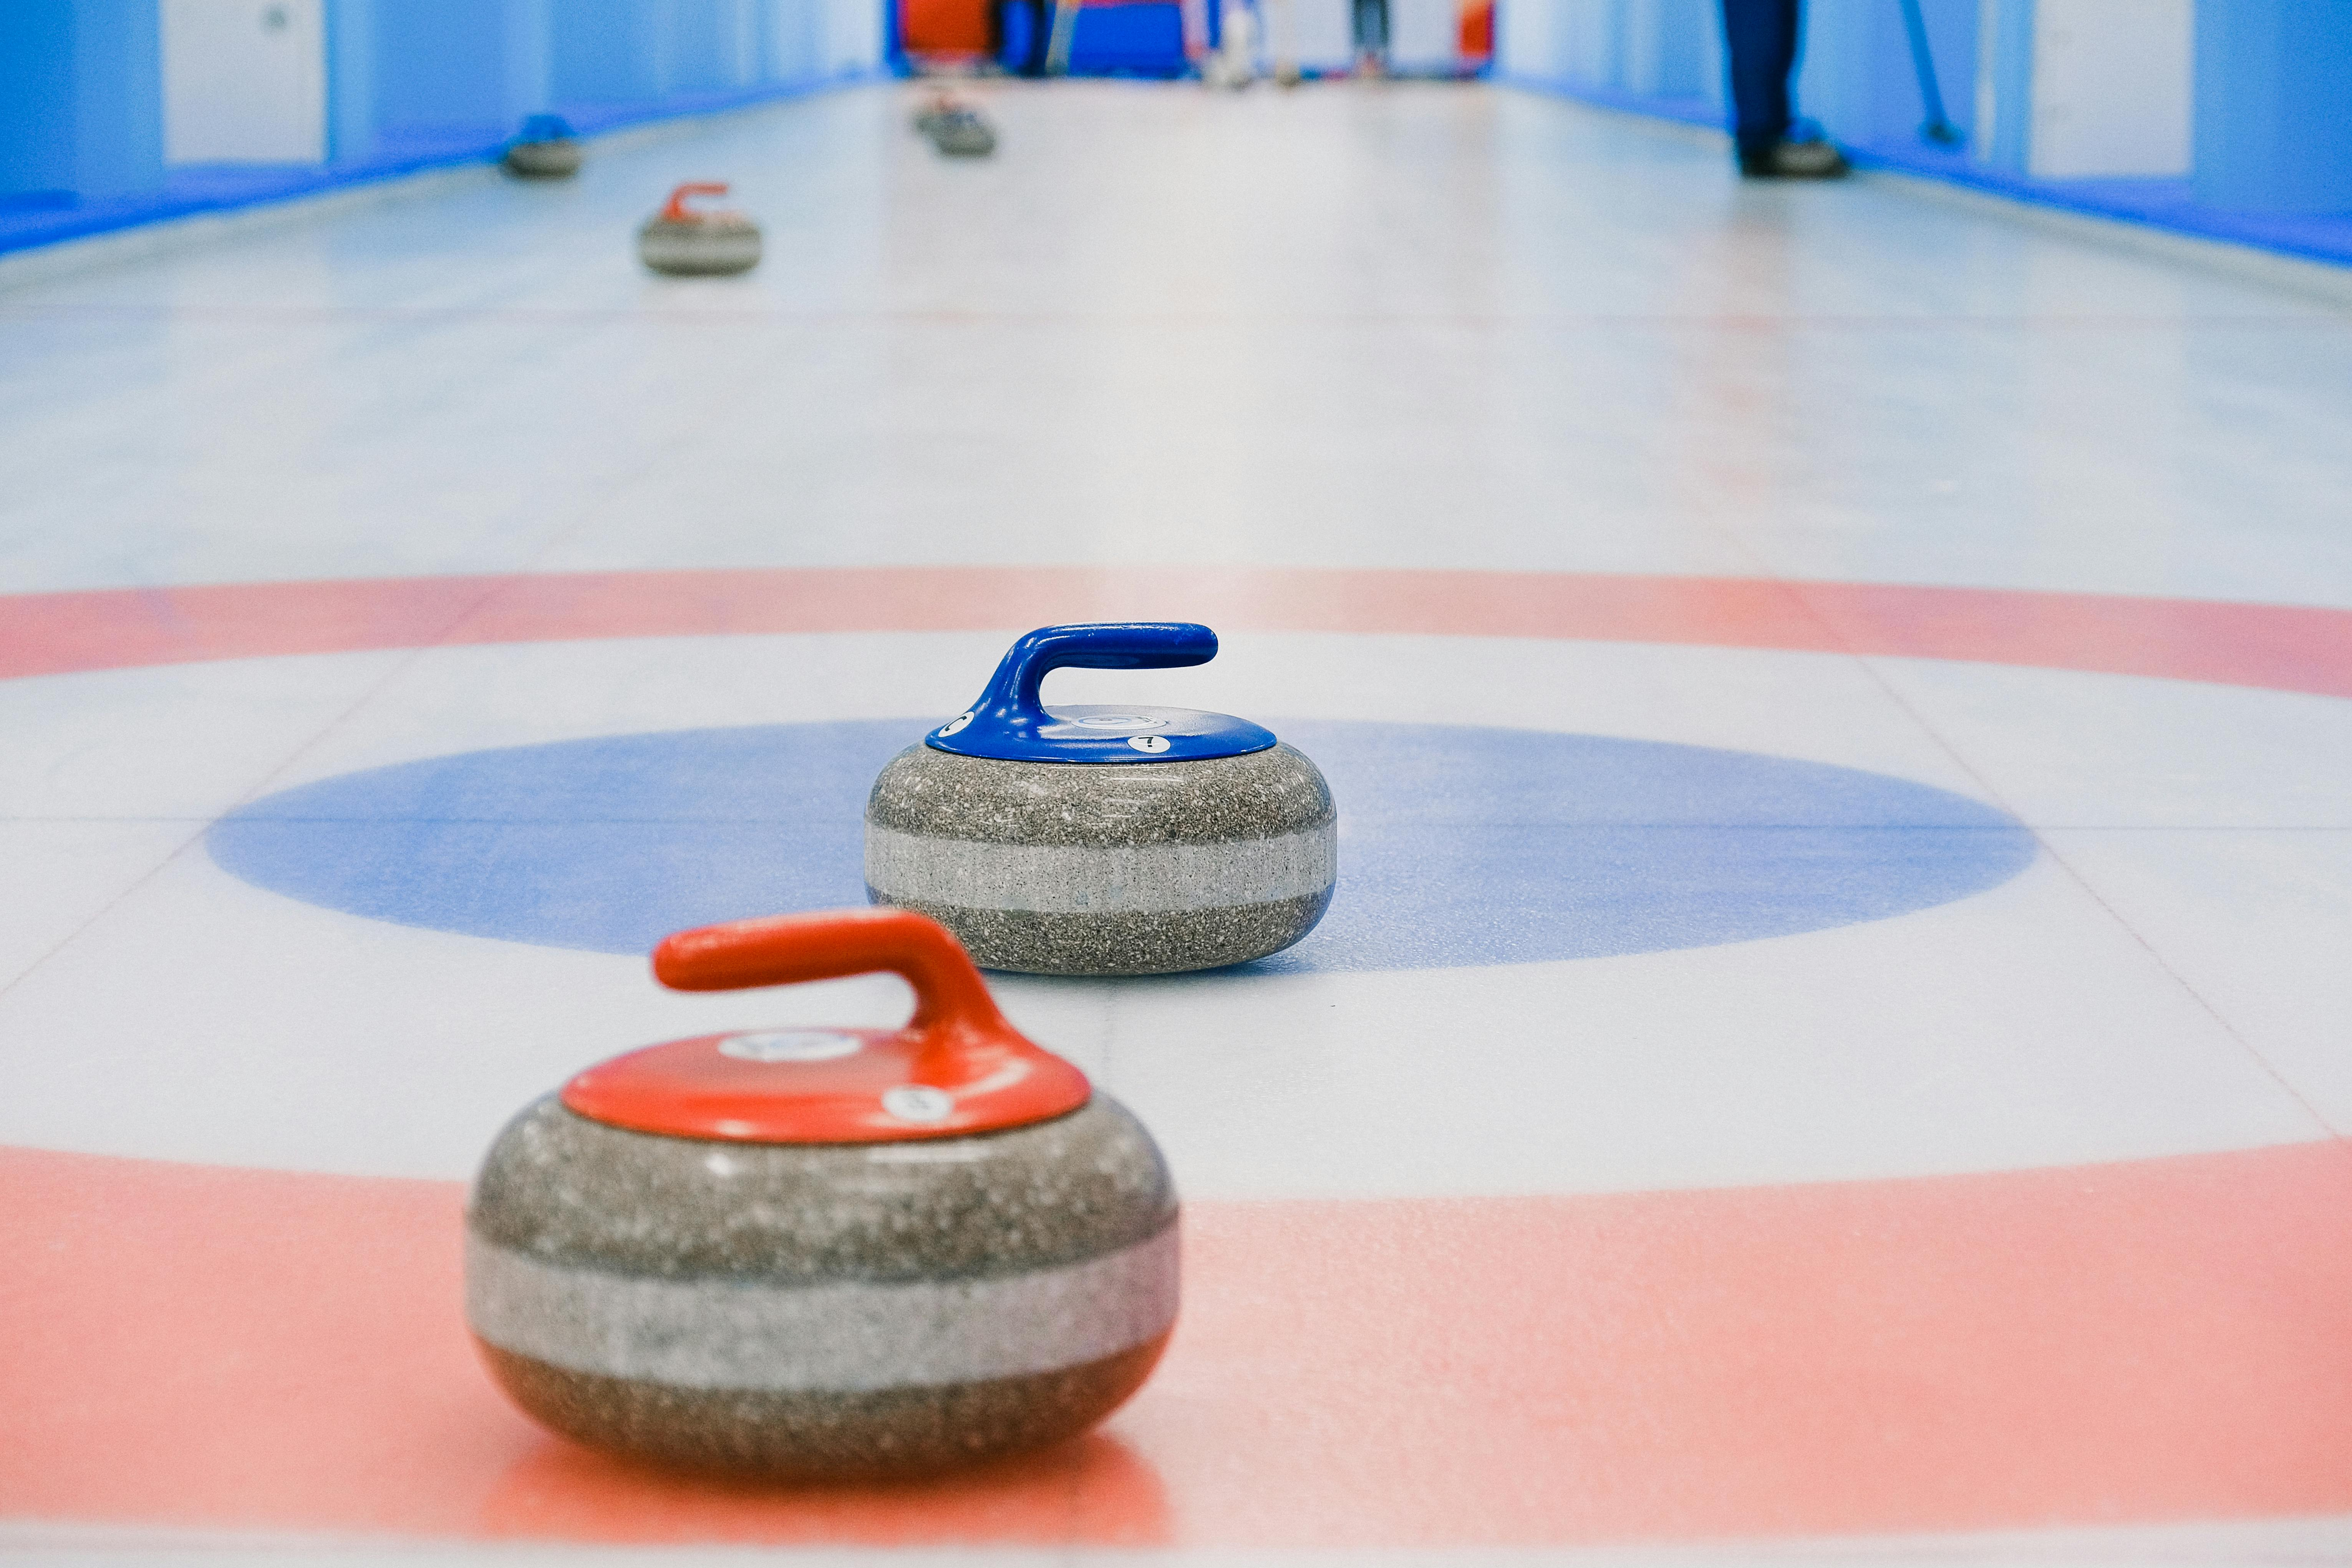
\includegraphics[height=4.1cm]{curling.jpg}
\end{center}





%%%%%%%%%%%

\subsection*{Reading}

Please read the following on your own in the OpenStax textbook by the dates given.  It will give good context for class discussion.  Check off when you have completed them.

\vspace{1em}

\begin{checkboxes}
  \choice 8.5 Inelastic Collisions in One
Dimension \dotfill \five
  \choice 8.6 Collisions of Point Masses in
Two Dimensions \dotfill \six
\end{checkboxes}


\subsection*{Problems and Conceptual Question}


Get stamps from your instructor as you complete each of the following problems.  The conceptual questions (CQ) require at least one sentence of explanation.

\vspace{1em}

\noindent
{\sc Stamps will not be given if work is not shown on a separate sheet of paper}

\vspace{1em}


\begin{tabular}{|*{3}{p{4.8cm}|}}
  \hline
  %
  \bs{Inelastic}{3}               
          & \bs{Two Dimensions}{3} 
          & \bs{Center of Mass}{4} \\
  Problems \#\ref{5p-i}-\ref{5p-f}
          & Problems \#\ref{6p-i}-\ref{6p-f} 
          & Problems \#\ref{7p-i}-\ref{7p-f}\\
  Conceptual \#\ref{5q-i}-\ref{5q-f}
          & %Conceptual \#\ref{6q-i}-\ref{6q-f}
          & %Conceptual \#\ref{7q-i}-\ref{7q-f} 
          \\
          & & \\[3em]\hline
  %%
\end{tabular}

\subsection*{Bonus Problems}

\hfill

\begin{tabular}{|*{4}{p{3.5cm}|}}
  \hline
  %
  \#\ref{b1}  &  \#\ref{b2}  &  \#\ref{b3} & \#\ref{b4}  \\[1.5cm]
  %
  \hline
\end{tabular}


%%%%%%%%%%%%%
%%%%%%%%%%%%%


\pagebreak 
\refsheet 
\pagebreak


\noindent
Questions and figures are from OpenStax \emph{College Physics}, 2nd ed, (Chapter 8) or Giancolli \emph{Physics: Principles with Applications}, 7th ed, (Chapter 7) unless otherwise noted.
 unless otherwise noted.



\begin{myquestions}

\myheading{Momentum \& Conservation}
\mysubheading{Problems}

% \myquestion (P1) 
% (a) Calculate the momentum of a 2000-kg elephant charging a hunter at a speed of 7.50~m/s. (b) Compare the elephant's momentum with the momentum of a 0.0400-kg tranquilizer dart fired at a speed of 600~m/s. (c) What is the momentum of the 90.0-kg hunter running at 7.40~m/s after missing the elephant?

\myquestion (P2) \label{1p-i}
(a) What is the mass of a large ship that has a momentum of \SI{1.60e9}{kg.m/s}, when the ship is moving at a speed of 48.0~km/h?  (b) Compare the ship's momentum to the momentum of a 1100-kg artillery shell fired at a speed of 1200~m/s.  ($\SI{3.6}{km/h}=\SI{1}{m/s}$) \answer{$m_\text{ship}=\SI{1.20e8}{kg}$; $p_\text{shell}=\SI{1.32e6}{kg.m/s}$}% $p_\text{ship}/p_\text{shell}=1,120$}

\myquestion (P3) 
(a) At what speed would a \num{2.00e4}-kg  airplane have to fly to have a momentum of \SI{1.60e9}{kg.m/s} (the same as the ship's momentum in the problem above)? (b) What is the plane's momentum when it is taking off at a speed of 60.0~m/s? (c) If the ship is an aircraft carrier that launches these airplanes with a catapult, discuss the implications of your answer to (b) as it relates to recoil effects of the catapult on the ship. \answer{(a) \SI{8.0e4}{m/s}; (b) \SI{1.20e6}{kg.m/s}}

\myquestion (P23)
\emph{Professional Application.} Train cars are coupled together by being bumped into one another. Suppose two loaded train cars are moving toward one another, the first having a mass of 150,000 kg and a velocity of 0.300 m/s, and the second having a mass of 110,000 kg and a velocity of $-0.120~$m/s. (The minus indicates direction of motion.) What is their final velocity? \answer{\SI{0.122}{m/s}}

\myquestion (Giancoli P7) 
A child in a boat throws a 5.30-kg package out horizontally with a speed of 10.0 m/s, Figure~\ref{7-31}. Calculate the velocity of the boat immediately after, assuming it was initially at rest. The mass of the child is 24.~ kg and the mass of the boat is 35.0~kg. \answer{0.90 m/s}

  \begin{figure}[H]
    \centering
    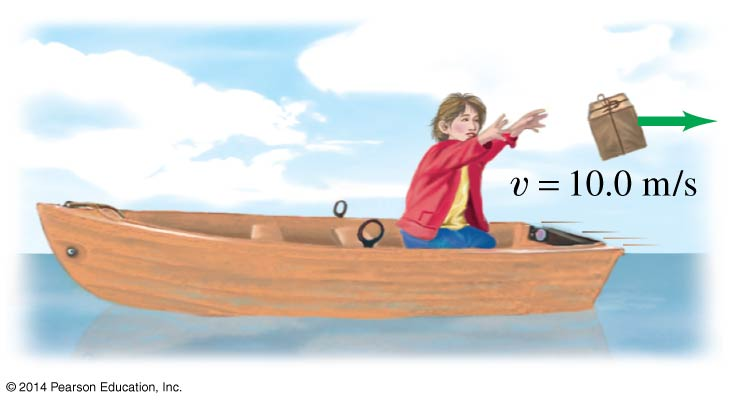
\includegraphics[width=5.5cm]{07_31_Figure.jpg}
    \caption{Giancolli Fig 7-31}
    \label{7-31}
  \end{figure}

\myquestion (P24)
Suppose a clay model of a koala bear has a mass of 0.200 kg and slides on ice at a speed of 0.750~m/s. It runs into another clay model, which is initially motionless and has a mass of 0.350 kg. Both being soft clay, they naturally stick together. What is their final velocity? \answer{\SI{0.272}{m/s}}

\myquestion (Giancolli P9, modified) \label{1p-f}
An atomic nucleus of mass 222~amu initially moving at 320~m/s emits an alpha particle of mass 4~amu in the direction of its velocity.  The remaining nucleus (of mass 218~amu) slows to a velocity of 280~m/s.  Find the velocity of the alpha particle.  (In nuclear chemistry, this process is the alpha decay of Radon-222: $^{222}_{86}\text{Rn} \rightarrow \text{}^{4}_{2}\alpha + \text{}^{218}_{84}\text{Po}$) \answer{2,500 m/s}




% \myquestion (P4) 
% (a) What is the momentum of a garbage truck that is \SI{1.20e4}{kg} and is moving at \SI{30.0}{m/s}? (b) At what speed would an 8.00-kg trash can have the same momentum as the truck?

% \myquestion (P26)
% What is the velocity of a 900-kg car initially moving at 30.0 m/s, just after it hits a 150-kg deer initially running at 12.0 m/s in the same direction? Assume the deer remains on the car.

% \myquestion (P27)
% A 1.80-kg falcon catches a 0.650-kg dove from behind in midair. What is their velocity after impact if the falcon's velocity is initially 28.0 m/s and the dove's velocity is 7.00 m/s in the same direction?

\mysubheading{Conceptual Questions}

\myquestion (CQ13, modified) \label{1q-i}
Is it possible for objects in a system to be moving even while the momentum of the system is zero? Explain your answer. 

\myquestion (Giancolli CQ9)
A boy stands on the back of a rowboat and dives into the water. What happens to the boat as he leaves it? Explain.

\myquestion (Giancoli MC1) 
A truck going 15 km/h has a head-on collision with a small car going 30 km/h. Which has a larger change in momentum? \answer{the momentum changes are the same (make sure to explain why)}

\myquestion (Giancoli MC2) A small boat coasts at constant speed under a bridge. A heavy sack of sand is dropped from the bridge onto the boat. What happens to the speed of the boat? Why? \answer{speed decreases (make sure to explain why)}

\myquestion (Giancoli MC4) \label{1q-f}
An astronaut is a short distance away from her space station without a tether rope. She has a large wrench. What should she do with the wrench to move toward the space station?


\myheading{Force \& Impulse}
\mysubheading{Problems}

\myquestion (P17) \label{2p-i}
Water from a fire hose is directed horizontally against a wall at a rate of 50.0 kg/s and a speed of 42.0 m/s. Calculate the magnitude of the force exerted on the wall, assuming the water's horizontal momentum is reduced to zero. \answer{\SI{2.10e3}{N}}

\myquestion (Giancolli P5) 
Calculate the force exerted on a rocket when the propelling gases are being expelled at a rate of \SI{1300}{kg/s} with a speed of \SI{4.5e5}{m/s}. \answer{\SI{5.85e7}{\newton}}


\myquestion (P7) 
A bullet is accelerated down the barrel of a gun by hot gases produced in the combustion of gun powder. What is the average force exerted on a 0.0300-kg bullet to accelerate it to a speed of 600.0 m/s in a time of 2.00 ms (milliseconds)?  ($\SI{1000}{ms}=\SI{1}{s}$) \answer{\SI{9000}{N}}


% \myquestion (P10) 
% \emph{Professional Application.} A professional boxer hits his opponent with a 1000-N horizontal blow that lasts for 0.150 s. (a) Calculate the impulse imparted by this blow. (b) What is the opponent's final velocity, if his mass is 105~kg and he is motionless in midair when struck near his center of mass? (c) Calculate the recoil velocity of the opponent's 10.0-kg head if hit in this manner, assuming the head does not initially transfer significant momentum to the boxer's body. (d) Discuss the implications of your answers for parts (b) and (c).

\myquestion (P11) \label{2p-f}
\emph{Professional Application.} Suppose a child drives a bumper car head on into the side rail, which exerts a force of 4000 N on the car for 0.200~s. (a) What impulse is imparted by this force? (b) Find the final velocity of the bumper car if its initial velocity was 2.80~m/s and the car plus driver have a mass of 200~kg. You may neglect friction between the car and floor. \answer{(a) \SI{-800}{N.s}; (b) \SI{-1.20}{m/s}}


% \myquestion(P18) 
% A 0.450-kg hammer is moving horizontally at 7.00 m/s when it strikes a nail and comes to rest after driving the nail 1.00 cm into a board. (a) Calculate the duration of the impact. (b) What was the average force exerted on the nail?

\myquestion \textbf{Bonus} (Giancoli P18) \label{b1}
A tennis ball of mass $m=0.060$~kg and speed $v=8$~m/s strikes a wall at a $45^\circ$ angle and rebounds with the same speed at $45^\circ$ (Figure~\ref{7-32}). What is the impulse (magnitude and direction) given to the ball? \answer{\SI{2.38}{N.s} to the left}

  \begin{figure}[H]
    \centering
    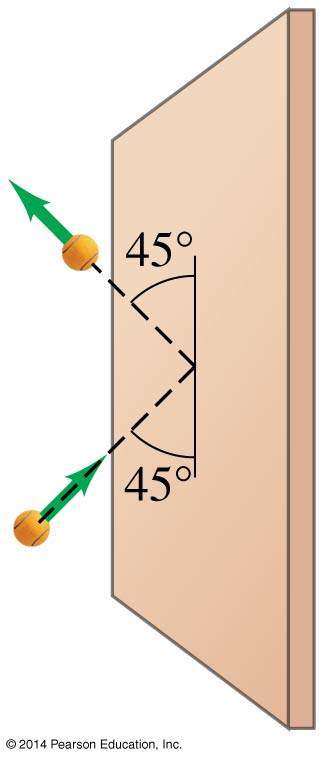
\includegraphics[height=5cm]{07_32_Figure.jpg}
    \caption{Giancolli Fig 7-32}
    \label{7-32}
  \end{figure}


\mysubheading{Conceptual Questions}

\myquestion (CQ4) \label{2q-i}
How could a small force impart the same momentum to an object as a large force?

\myquestion (CQ5) \emph{Professional Application.}
Explain in terms of impulse how padding reduces forces in a collision. State this in terms of a real example, such as the advantages of a carpeted vs. tile floor for a day care center.

\myquestion (Giancolli CQ15)
Cars used to be built as rigid as possible to withstand collisions. Today, though, cars are designed to have "crumple zones" that collapse upon impact. What is the advantage of this new design?

\myquestion (Giancoli MC7) \label{2q-f}
You are lying in bed and want to shut your bedroom door. You have a bouncy ball and a blob of clay, both with the same mass. Which one would be more effective to throw at your door to close it? \answer{bouncy ball (make sure to explain why)}




\myheading{Elastic Collisions}
\mysubheading{Problems}


% \myquestion (P28)
% Two identical objects (such as billiard balls) have a one-dimensional collision in which one is initially motionless. After the collision, the moving object is stationary and the other moves with the same speed as the other originally had. Show that both momentum and kinetic energy are conserved.


\myquestion (Giancolli P25) \label{4p-i}
A ball of mass 0.440 kg moving east ($+x$ direction) with a speed of 3.80~m/s collides head-on with a 0.220-kg ball at rest. If the collision is perfectly elastic, what will be the speed and direction of each ball after the collision? \answer{1.27 m/s;  5.07 m/s}

\myquestion (Giancolli P26) A 0.450-kg hockey puck, moving east with a speed of 5.80~m/s, has a head-on collision with a 0.900-kg puck initially at rest. Assuming a perfectly elastic collision, what will be the speed and direction of each puck after the collision? \answer{$-1.93$ m/s;  3.87 m/s}


% \myquestion (P29)
% \emph{Professional Application.} Two piloted satellites approach one another at a relative speed of 0.250 m/s, intending to dock. The first has a mass of \SI{4.00e3}{kg}, and the second a mass of \SI{7.50e3}{kg}. If the two satellites collide elastically rather than dock, what is their final relative velocity?

\myquestion (P30) \label{4p-f}
A 70.0-kg ice hockey goalie, originally at rest, catches a 0.150-kg hockey puck slapped at him at a velocity of 35.0 m/s. Suppose the goalie and the ice puck have an elastic collision and the puck is reflected back in the direction from which it came. What would their final velocities be in this case? \answer{\SI{-34.9}{m/s}; \SI{0.150}{m/s}}


\mysubheading{Conceptual Questions}

\myquestion (CQ15) \label{4q-i}
What is an elastic collision?

\myquestion (Giancoli MC12) \label{4q-f}
A bowling ball hangs from a 1.0-m-long cord, Figure~\ref{7-30}: (i) A 200-gram putty ball moving 5.0 m/s hits the bowling ball and sticks to it, causing the bowling ball to swing up; (ii) a 200-gram rubber ball moving 5.0~m/s hits the bowling ball and bounces straight back at nearly 5.0~m/s, causing the bowling ball to swing up.  In which case (if either) will the bowling ball swing higher up? \answer{(ii) will go higher (make sure to explain why)}

  \begin{figure}[H]
    \centering
    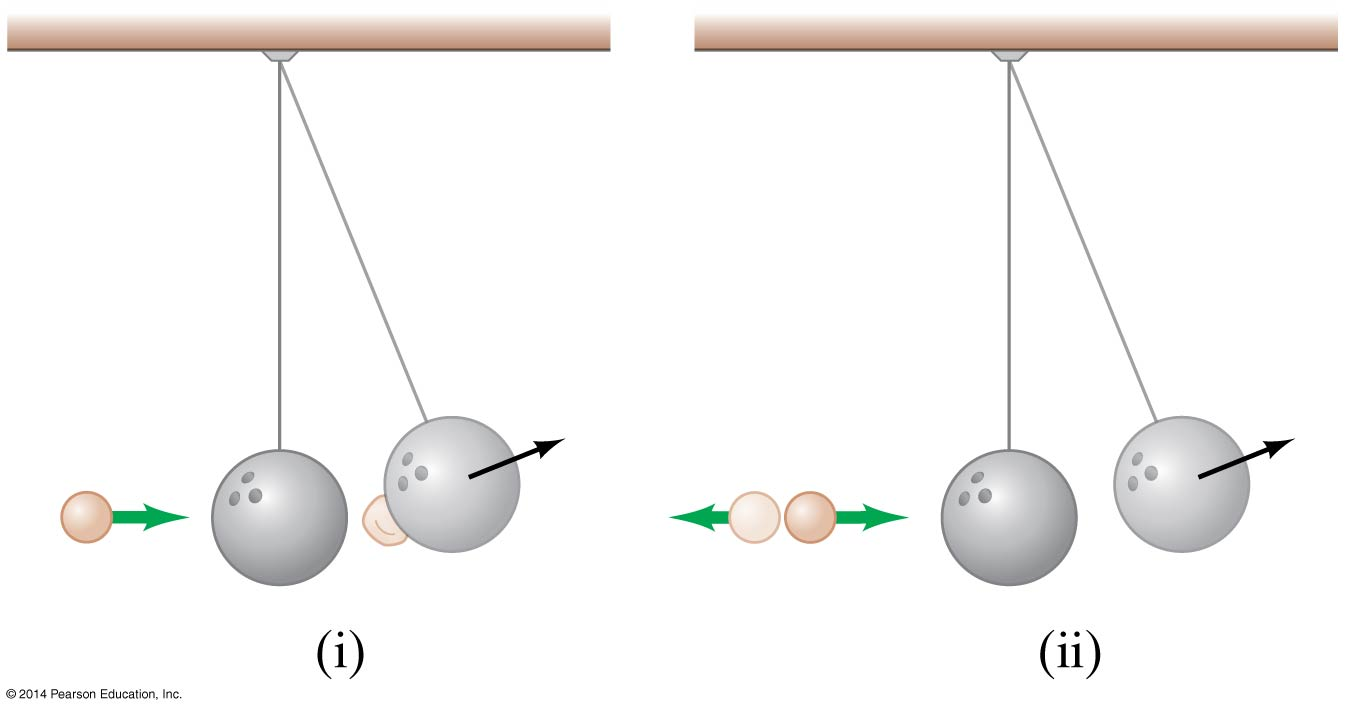
\includegraphics[width=5.5cm]{07_30_Figure.jpg}
    \caption{Giancolli Fig 7-30}
    \label{7-30}
  \end{figure}




  

\myheading{Inelastic Collisions}
\mysubheading{Problems}

\myquestion (P32) \label{5p-i}
During an ice show, a 60.0-kg skater leaps into the air and is caught by an initially stationary 75.0-kg skater. (a) What is their final velocity assuming negligible friction and that the 60.0-kg skater's original horizontal velocity is 4.00 m/s? (b) How much kinetic energy is lost? \answer{(a)\SI{1.78}{m/s}; (b) \SI{-267}{J}}

\myquestion (P34) \label{5p-f}
A battleship that is \SI{6.00e7}{kg} and is originally at rest fires a 1100-kg artillery shell horizontally with a velocity of 575 m/s. (a) If the shell is fired straight aft (toward the rear of the ship), there will be negligible friction opposing the ship's recoil. Calculate its recoil velocity. (b) Calculate the increase in internal kinetic energy (that is, for the ship and the shell). \emph{This energy is less than the energy released by the gun powder—significant heat transfer occurs.} \answer{(a) \SI{-0.0105}{m/s}; (b) \SI{1.818e8}{J}}

% \myquestion (P39)
% \emph{Professional Application.} One of the waste products of a nuclear reactor is plutonium-239 ($^{239}\text{Pu}$). This nucleus is radioactive and decays by splitting into a helium-4 nucleus and a uranium-235 nucleus \mbox{($^4\text{He}+^{235}\text{U}$)}, the latter of which is also radioactive and will itself decay some time later. The energy emitted in the plutonium decay is \SI{8.40e-13}{J} and is entirely converted to kinetic energy of the helium and uranium nuclei. The mass of the helium nucleus is \SI{6.68e-27}{kg}, while that of the uranium is \SI{3.92e-25}{kg} (note that the ratio of the masses is 4 to 235). (a) Calculate the velocities of the two nuclei, assuming the plutonium nucleus is originally at rest. (b) How much kinetic energy does each nucleus carry away? Note that the data given here are accurate to three digits only.

% \myquestion (P41)
% \emph{Professional Application.} Two football players collide head-on in midair while trying to catch a thrown football. The first player is 95.0 kg and has an initial velocity of 6.00 m/s, while the second player is 115 kg and has an initial velocity of $-3.50$~m/s. What is their velocity just after impact if they cling together?

% \myquestion (P42)
% What is the speed of a garbage truck that is \SI{1.20e4}{kg}  and is initially moving at 25.0~m/s just after it hits and adheres to a trash can that is 80.0~kg and is initially at rest?

\myquestion \textbf{Bonus} (P40) \label{b2}
\emph{Professional Application.} The Moon's craters are remnants of meteorite collisions. Suppose a fairly large asteroid that has a mass of \SI{5.00e12}{kg}  (about a kilometer across) strikes the Moon at a speed of 15.0~km/s. (a) At what speed does the Moon recoil after the perfectly inelastic collision (the mass of the Moon is \SI{7.36e22}{kg})? (b) How much kinetic energy is lost in the collision? Such an event may have been observed by medieval English monks who reported observing a red glow and subsequent haze about the Moon. (c) In October 2009, NASA crashed a rocket into the Moon, and analyzed the plume produced by the impact. (Significant amounts of water were detected.) Answer part (a) and (b) for this real-life experiment. The mass of the rocket was 2000 kg and its speed upon impact was 9000 km/h. How does the plume produced alter these results?

\myquestion \textbf{Bonus} (Giancolli Additional Practice Problem 3) \label{b3}
In a physics lab, a cube slides down a frictionless incline as shown in Figure~\ref{7-50} and elastically strikes another cube at the bottom that is only one-half its mass. If the incline is 35~cm high and the table is 95~cm off the floor, where does each cube land? [\emph{Hint:} Both leave the incline moving horizontally.]

  \begin{figure}[H]
    \centering
    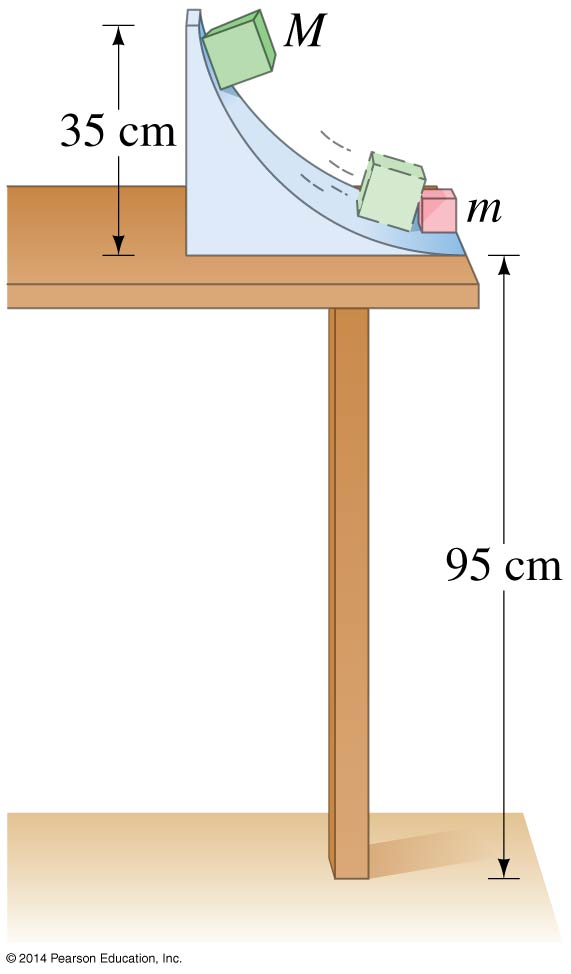
\includegraphics[height=6cm]{07_50_Figure.jpg}
    \caption{Giancolli Fig 7-50}
    \label{7-50}
  \end{figure}




\mysubheading{Conceptual Questions}

\myquestion (CQ16) \label{5q-i}
What is an inelastic collision? What is a perfectly inelastic collision?

\myquestion (CQ17) \label{5q-f}
Mixed-pair ice skaters performing in a show are standing motionless at arm's length just before starting a routine. They reach out, clasp hands, and pull themselves together by only using their arms. Assuming there is no friction between the blades of their skates and the ice, what is their velocity after their bodies meet? \answer{0 m/s (make sure to explain why)}


\myheading{Collisions of Point Masses in Two Dimensions}
\mysubheading{Problems}

\myquestion (P50) \label{6p-i}
\emph{Professional Application.} Two cars collide at an icy intersection and stick together afterward. The first car has a mass of 1200~kg and is approaching at 8.00~m/s  due south. The second car has a mass of 850 kg and is approaching at 17.0~m/s  due west. (a) Calculate the final velocity (magnitude and direction) of the cars. (b) How much kinetic energy is lost in the collision? (This energy goes into deformation of the cars.) \answer{(a) \SI{8.46}{m/s} @ $33.6^\circ$ S of W; (b) \SI{-8.78e4}{J}}

% \myquestion (P45)
% Two identical pucks collide on an air hockey table. One puck was originally at rest. (a) If the incoming puck has a speed of 6.00~m/s and scatters to an angle of $30.0^\circ$,what is the velocity (magnitude and direction) of the second puck? (You may use the result that $\theta_1-\theta_2=90^\circ$  for elastic collisions of objects that have identical masses.) (b) Confirm that the collision is elastic.

% \myquestion (P47)
% A 3000-kg cannon is mounted so that it can recoil only in the horizontal direction. (a) Calculate its recoil velocity when it fires a 15.0-kg shell at 480 m/s at an angle of $20.0^\circ$ above the horizontal. (b) What is the kinetic energy of the cannon? This energy is dissipated as heat transfer in shock absorbers that stop its recoil. (c) What happens to the vertical component of momentum that is imparted to the cannon when it is fired?

\myquestion (P48) \label{6p-f}
\emph{Professional Application.} A 5.50-kg bowling ball moving at 9.00 m/s collides with a 0.850-kg bowling pin, which is scattered at an angle of $85.0^\circ$ to the initial direction of the bowling ball and with a speed of 15.0 m/s.  Calculate the final velocity (magnitude and direction) of the bowling ball. %(b) Is the collision elastic? (c) Linear kinetic energy is greater after the collision. Discuss how spin on the ball might be converted to linear kinetic energy in the collision.
\answer{\SI{9.10}{m/s} @ $-14.7^\circ$}


\myheading{Center of Mass}
\mysubheading{Problems}

\myquestion (Giancoli P50) \label{7p-i}
Find the center of mass of the three-mass system shown in Figure~\ref{7-37} relative to the 1.00-kg mass. \answer{0.44 m}

  \begin{figure}[H]
    \centering
    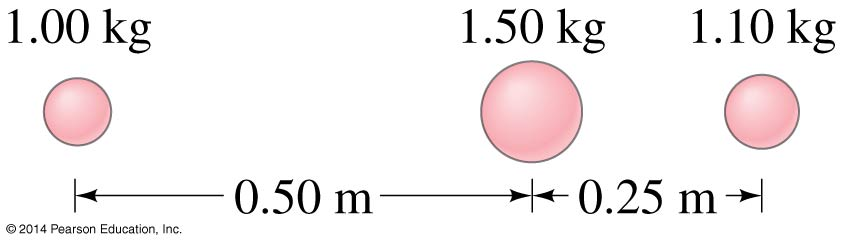
\includegraphics[width=6.1cm]{07_37_Figure.jpg}
    \caption{Giancolli Fig 7-37}
    \label{7-37}
  \end{figure}

\myquestion (Giancoli P49) 
The distance between a carbon atom ($m=\SI{12}{amu}$) and an oxygen atom ($m=\SI{16}{amu}$ in the CO molecule is \SI{1.13e-10}{m}. How far from the carbon atom is the center of mass of the molecule? \answer{\SI{6.46e-11}{\meter}}


% \myquestion (Giancoli P51)
% The {\sc cm} of an empty 1250-kg car is 2.40~m behind the front of the car. How far from the front of the car will the {\sc cm} be when two people sit in the front seat 2.80~m from the front of the car, and three people sit in the back seat 3.90~m from the front? Assume that each person has a mass of 65.0~kg. \answer{2.61 m from front of car}
 
\myquestion (Giancoli P52) \label{7p-f}
Three cubes, of side $\ell_0$, $2\ell_0$, and $3\ell_0$, are placed next to one another (in contact) with their centers along a straight line as shown in Figure~\ref{7-38}. What is the position, along this line, of the CM of this system? Assume the cubes are made of the same uniform material. \answer{$x_\text{\sc cm}=3.8\ell_0$}

  \begin{figure}[H]
    \centering
    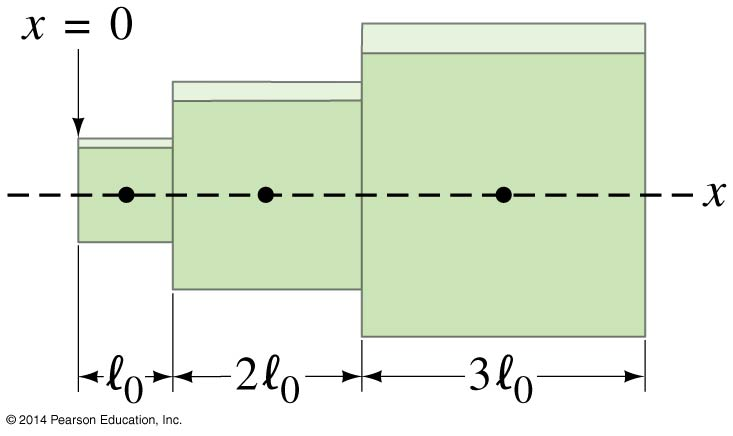
\includegraphics[width=5cm]{07_38_Figure.jpg}
    \caption{Giancolli Fig 7-38}
    \label{7-38}
  \end{figure}

\myquestion \textbf{Bonus} (Giancolli P55) \label{b4}
A uniform circular plate of radius $2R$ has a circular hole of radius $R$ cut out of it. The center C' of the smaller circle is a distance $0.80R$ from
the center C of the larger circle, Figure~\ref{7-41}. What is the position of the center of mass of the plate? [\emph{Hint:} Try subtraction.] \answer{$0.27R$ left of the center}

  \begin{figure}[H]
    \centering
    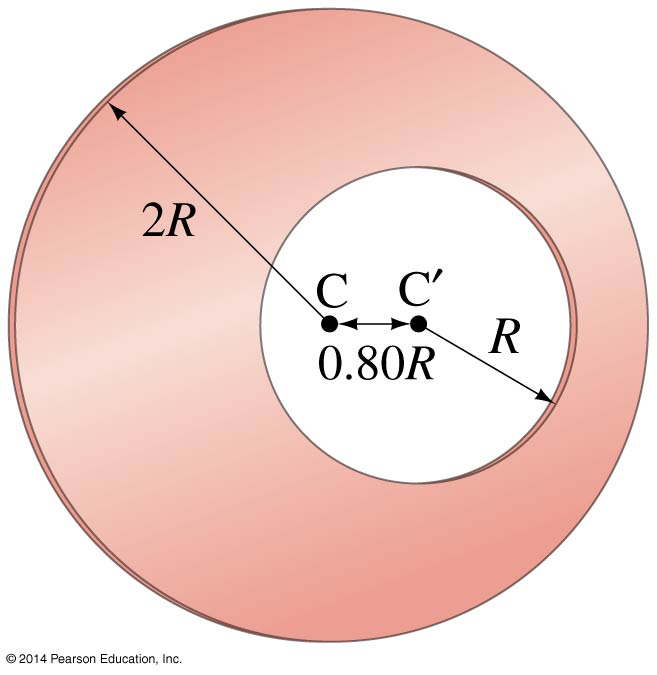
\includegraphics[width=5cm]{07_41_Figure.jpg}
    \caption{Giancolli Fig 7-41}
    \label{7-41}
  \end{figure}



\end{myquestions}

\end{document}